te\chapter{Kern der Arbeit}

\anno{ca. 15-20 Seiten}

% Probleme und die Loesungsansaetze
\section{Probleme}

Der im vorherigen Kapitel betrachtete zeitliche Rahmen, über die Entwicklung von Web Application Firewalls, umfasst mehr als zwanzig Jahre. Ein Zeitraum in dem sich zahlreiche Produkte in diesem Bereich etablierten. Im Anhang finden Sie, beispielsweise, unter \ref{tab:my_wafwoof} eine (nicht vollständige) Liste von derzeitigen WAF-Produkten verschiedener Hersteller. Über den gesamten Zeitraum haben sich Webtechnologien weiterentwickelt und auch die Art und Weise der Nutzungs des Internets änderte sich. Mit der Verbreitung der Smartphones und Sprachassistenten wurden aus einfachen Webangeboten vielschichtige Anwendungen mit verschiedenen möglichen Clientsystemen (\emph{mobile-first-Ansatz}). Serviceorientierte Architekturen, Webservices, Microservices, Künstliche Intelligenz - alles entwickelte sich weiter. Im Bereich der IT-Sicherheit veröffentlichte das \emph{Open Web Application Security Project} 2019 erstmals eine Liste seiner zehn kritischsten Sicherheitsrisiken explizit für den Bereich der \emph{API}s. \emph{ModSecurity} ist immernoch der defacto-Standart für regelbasierte WAFs und praktisch so gut wie der einzige verbliebene Vertreter der Web Application Firewalls aus dem OpenSource-Bereich. Freie anomaliebasierte Systeme sind so gut wie nicht existent und die privatwirtschaftlichen Akteure lassen sich kaum in die Karten schauen. \\
Mittlerweile sind bereits dreizehn Jahre seit dem Erscheinen des Datensatzes CSIC2010 vergangen und schaut man in die derzeitig vorhandene Literatur scheint auch kein Nachfolger in Sicht. \\\\

\textcolor{bhtGray}{\ding{110} Applebaum über den Datensatz CSIC2010~\cite{Applebaum2021}} Gimenéz et al. provide an HTTP dataset intended to be used for the development and testing of Intrusion Detections Systems and WAFs. ... The dataset has been used extensively by other researchers ... There is still a need for a development of a new dataset as previous datasets had become outdated and did not target real systems. The dataset .. is itself now over 10 years old and targets a bespoke e-commerce system. \\\\


%

\subsection{Aufbau des Datensatzes CSIC2010}

% Aufbau /motivation von gimenez

% Aufbau
Der Datensatz besteht aus drei Teildatensätzen. Der erste Teildatensatz ist dabei für die Trainingsphase gedacht und enthält nur den normalen Datenverkehr. Die anderen beiden Teildatensätze sind für die Testphase gedacht, ein Teildatensatz mit normalem Datenverkehr und ein Teildatensatz mit \emph{bösartigem} Daten (siehe \cite{csic2010}). Die einzelnen Dateneinträge der drei Teildatensätze sind gleich aufgebaut und beinhalten

\begin{description}
\item[HTTP Methode] \verb=GET= oder \verb=POST= im Anomalieteil auch \verb=PUT=
\item[URL]
\item[Protocol]
\item[User-Agent]
\item[Pragma]
\item[Cache-control]
\item[Accept]
\item[Accept-Encoding]
\item[Accept-Charset]
\item[Accept-Language]
\item[Host]
\item[Cookie]
\item[Content-Type]
\item[Connection]
\item[ContentLength]
\end{description}




\subsection{Alter des Datensatzes}

\subsubsection{Das HTTP-Protokoll}

%% Erweiterung HTTP
\subsubsection{Neue Anwendungsarchitekturen}
%% Änderungen Anwendungsarchitekturen

\subsection{Ziel des Datensatzes}

Erhöhung der allgemeinen Gültigkeit (Diskrepanz mit spezieller Zuschneidung auf Anwendung)
Erhöhung der Genauigkeit

% SChönes Beispiel für Fortschritt, produktiven Einsatz und zeitliche Veränderung und wo Gimenez nicht funktioniert-- > PUT als anomalie in CSIC2010 definiert aber in REST durchaus üblich
% rest beispiel mit PUT

%\lstset{language=XML,
% 	basicstyle=\ttfamily\color{black}\small,
% 	keywordstyle=\bfseries\color{bhtBlue},
% 	identifierstyle=\color{black}, 
% 	commentstyle=\color{gray}\textsl
%      }
      \begin{figure}
        \caption{Beispiel für einfachen REST-Request}
        \label{fig:restputexample}
      \begin{lstlisting}
PUT /user/devtty HTTP/1.1
Host: petstore.devtty.de
Content-Type: application/json

{
  "id": 2334,
  "username": devtty,
  "firstName": "Denis",
  "lastName": "Renning"
}
\end{lstlisting}
\end{figure}



% Methodik und Vorgehen
\section{Methodik}

% Uebersicht Architektur

\section{Lösungen}

\subsection{Unzureichende Kategorisierung im Datensatz}
% Problem zu viele Falsch-Positive/Zuordnung:Framework/Status(Session) -> Anwendungsstatus (DeltaspikeClientId/SpringExecuteID)
% möglichkeit anomalien nicht auf basis der Regeln sondern auf basis von abweichungen in der Anwendungsnutzung auszuwerten

% Erweiterung Datenset um Variablen (eingeloggt/framework/id)

\begin{figure}[ht]
  \begin{center}
    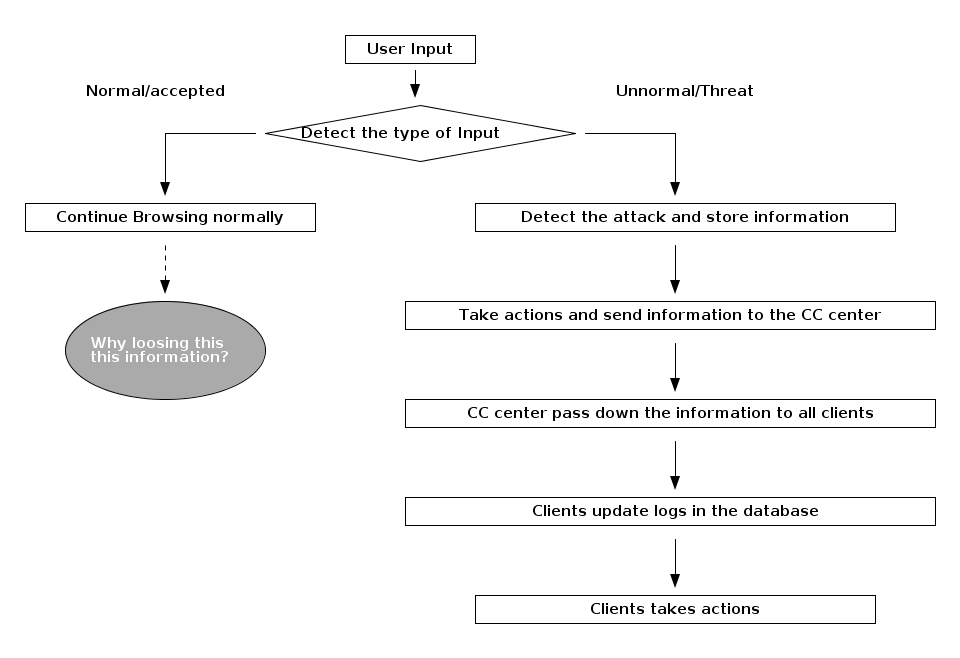
\includegraphics[width=15cm]{waf_mana}
    \caption{Zentralisiert~\cite{Manaseer2018}}
    \label{fig.topten}
  \end{center}
\end{figure}


% Oder: Der xxx Algorithmus

% Oder: Der yyy Algorithmus

% Zusammenfassung: ca. 0,5 Seiten
\section{Zusammenfassung}

\begin{neu}
  Anfang mit Aufnahme des Altenbestands, hinzufügen Entwicklungsumgebung, Test, etc

  Entwicklung Zentrale Steuerung

  Entwicklung ML Anteil
\end{neu}